%----------------------------------------------------------------------------------------
\section{ZigBee}
%----------------------------------------------------------------------------------------
\subsection{ZigBee standard}
%----------------------------------------------------------------------------------------
At the moment ZigBee is the leading protocol to implement low-cost low-data-rate, short-range WSNs. It is an open global standard built on IEEE 802.15.4 and provides extra functionality regarding advanced routing capabilities and network stability.
%-----------------------------------------
\subsection{ZigBee stack}
A common concept used to simplify and make digital communication more flexible, is the use of networking layers. Each layer is responsible for certain specific functions and pass data and commands only to the layers directly above or below via service access points. Figure \ref{fig:stack} shows how this is organized in the ZigBee protocol stack.  The bottom two layers are defined by the IEEE 802.15.4 standard and define the specifications for PHY and MAC layers. ZigBee only defines the networking, application and security layer on top of IEEE 802.15.4.\\
\begin{figure}[htbp]
\centering
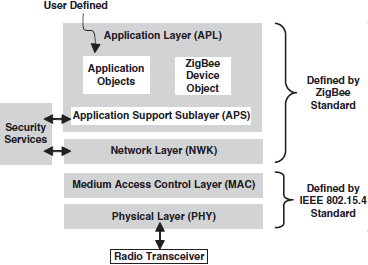
\includegraphics[width=0.48\textwidth]{stack}
%\rule{30em}{0.5pt}
\caption{ZigBee Protocol Layers}
\label{fig:stack}
\end{figure} 
\paragraph{PHY Layer Responsibilities}
\begin{itemize}
\item Enabling and disabling the radio transceiver ... ...
\item Transmit and receive data ... ...
\item Select CH ... ...
\item Estimating signal energy ... ...
\item Providing RSSI, LQI ... ...
\end{itemize}
\paragraph{MAC Layer Responsibilities}
\begin{itemize}
\item Generating beacons ... ...
\item CSMA-CA, BPSK vs. O-QPSK, vs. ASK ... ...
\item Providing a reliable link ... ...
\item PAN association and disassociation services
\end{itemize}
\paragraph{Network Layer Responsibilities}
\begin{itemize}
\item Setting up a network ... ...
\item Allow joining and leaving a network ... ...
\item Configuring new devices ... ...
\item Discover and maintain routes ... ...
\end{itemize}
\paragraph{Application Layer Responsibilities}
\begin{itemize}
\item Application support ... ...
\item Address management and mapping ... ...
\item Define the role of the device ... ...
\item Security related tasks ... ...
\end{itemize}
%-----------------------------------------
\subsection{Networking concepts}
\subsubsection{Device Types}
\subsubsection{Device Roles}
\paragraph{Coordinator Operation}
\paragraph{Router Operation}
\paragraph{End Device Operation}
sleep...
\subsection{Parent - Child relationship}
%-------------------------------------------------------------------
\subsection{API Frame Specifications}
To communicate with the ZigBee radio there are 2 modes, AT (transparent mode) and API (application programming interface). AT mode means that what you send to the zigbee radio using RS232, the ZigBee radio will send to its default destination. Unless you send “+++”, wait for the ZigBee to reply with OK, and then send an AT command. AT commands are used to change the configuration of the ZigBee radio. For instance the AT command OP requests the operating PAN ID.\\
AT mode is fairly limited and only good for point to point communication since you can’t really specify the destination unless you change the default destination all the time. So that is why the sensor network operates in API mode. This means that everything sent to the zigbee radio, using serial communication, is now packetized.\\
API defines a number of different packets as can be found in chapter 9 of \defcitealias{XBEE}{XBee/XBee-Pro ZB RF Modules User Manual, 2012}\citepalias{XBEE}. An API packet is shown in figure \ref{fig:api}. It starts with 0x7E as start delimiter and is followed by the length of the data excluding checksum. Then a API-specific structure follow which depends on the type of packet.\\
\begin{figure}[htbp]
\centering
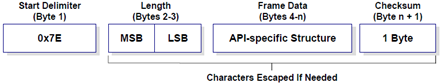
\includegraphics[width=0.48\textwidth]{api}
\caption{UART Data Frame Structure}
\label{fig:api}
\end{figure} 
\begin{table}[!ht]
\begin{center}
\begin{tabular}[!ht]{|c|c|}
\hline
\textbf{API Frame Name} & \textbf{API ID}\\
\hline
AT Command & 0x08\\
\hline
ZigBee Transmit Request & 0x10\\
\hline
AT Command Response & 0x88\\
\hline
ZigBee Receive Packet & 0x90\\
\hline
\end{tabular}
\caption{API Frame Names and Values}
\label{tab:apis}
\end{center}
\end{table}\\
\label{api1}\noindent
A reduced list of possible packets can be found in table \ref{tab:apis} (for the full list please see appendix \ref{AppendixF}). As mentioned an AT command is used to alter configurations of the ZigBee radio. This can of course also be done in API mode. For details about all the packets, please consult the datasheet. The only packets types used in this project are: 'ZigBee transmit request, 0x10' and 'Zigbee receive packet, 0x90'.\\
A ZigBee transmit request is shown in figure \ref{fig:api4}. This packet is used to send data from this ZigBee radio to a remote one. All that has to be known is the remote ZigBee address. These types of packets are constructed by the gateway to send out data to the libelium nodes but also by libelium nodes to send data to other libelium nodes or the gateway. Libelium has its own specific format for the RF Data as will be explained in section \ref{libPAQ}. To reach the gateway the address of the coordinator can be used, since the coordinator and gateway in our case are the same. This is convenient since the coordinator can always be addressed with 0x0000000000000000. The reason we chose the gateway and coordinator to be the same is that the coordinator receives a lot of traffic due to its role as coordinator and the same goes for the gateway. So these 2 devices should be in the center of the network for efficiency reasons. Assigning one device for these 2 roles and trying to position this device as central as possible will ask for the least amount of routing overhead.\\
When data is received by a ZigBee radio, this radio will send out a Zigbee receive packet via its serial communication. An example of this packet can be found in figure \ref{fig:api5}. Again the received data has an additional format as specified by Libelium.
\vfill 